\chapter{Introduzione}

Negli ultimi anni i dispositivi indossabili per la registrazione di video in prima persona hanno conosciuto una diffusione sempre più ampia. Strumenti come \emph{smart glasses}, \emph{body cameras}, \emph{action cameras} hanno reso possibile la cattura di flussi visivi continui dal punto di vista diretto dell'utilizzatore, dando origine a quella che viene comunemente definita come \emph{egocentric video}. Questa modalità di acquisizione ha suscitato un forte interesse \cite{NUNEZMARCOS2022175} non solo per le applicazioni pratiche, che spaziano dallintrattenimento personale alla sicurezza e al monitoraggio di attività lavorative, ma anche per le sfide che pone in termini di analisi e interpretazione dei contenuti.

\begin{figure}[ht]
    \centering
    \begin{minipage}{0.3\linewidth}
        \centering
        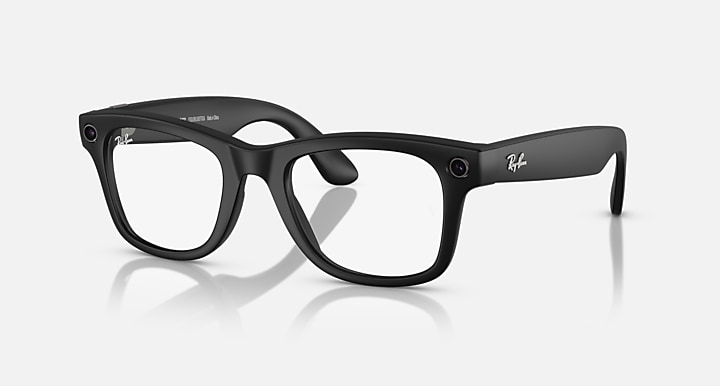
\includegraphics[width=\linewidth]{Images/meta_glass.png}\\
        (a) Smart glasses
    \end{minipage}
    \hfill
    \begin{minipage}{0.3\linewidth}
        \centering
        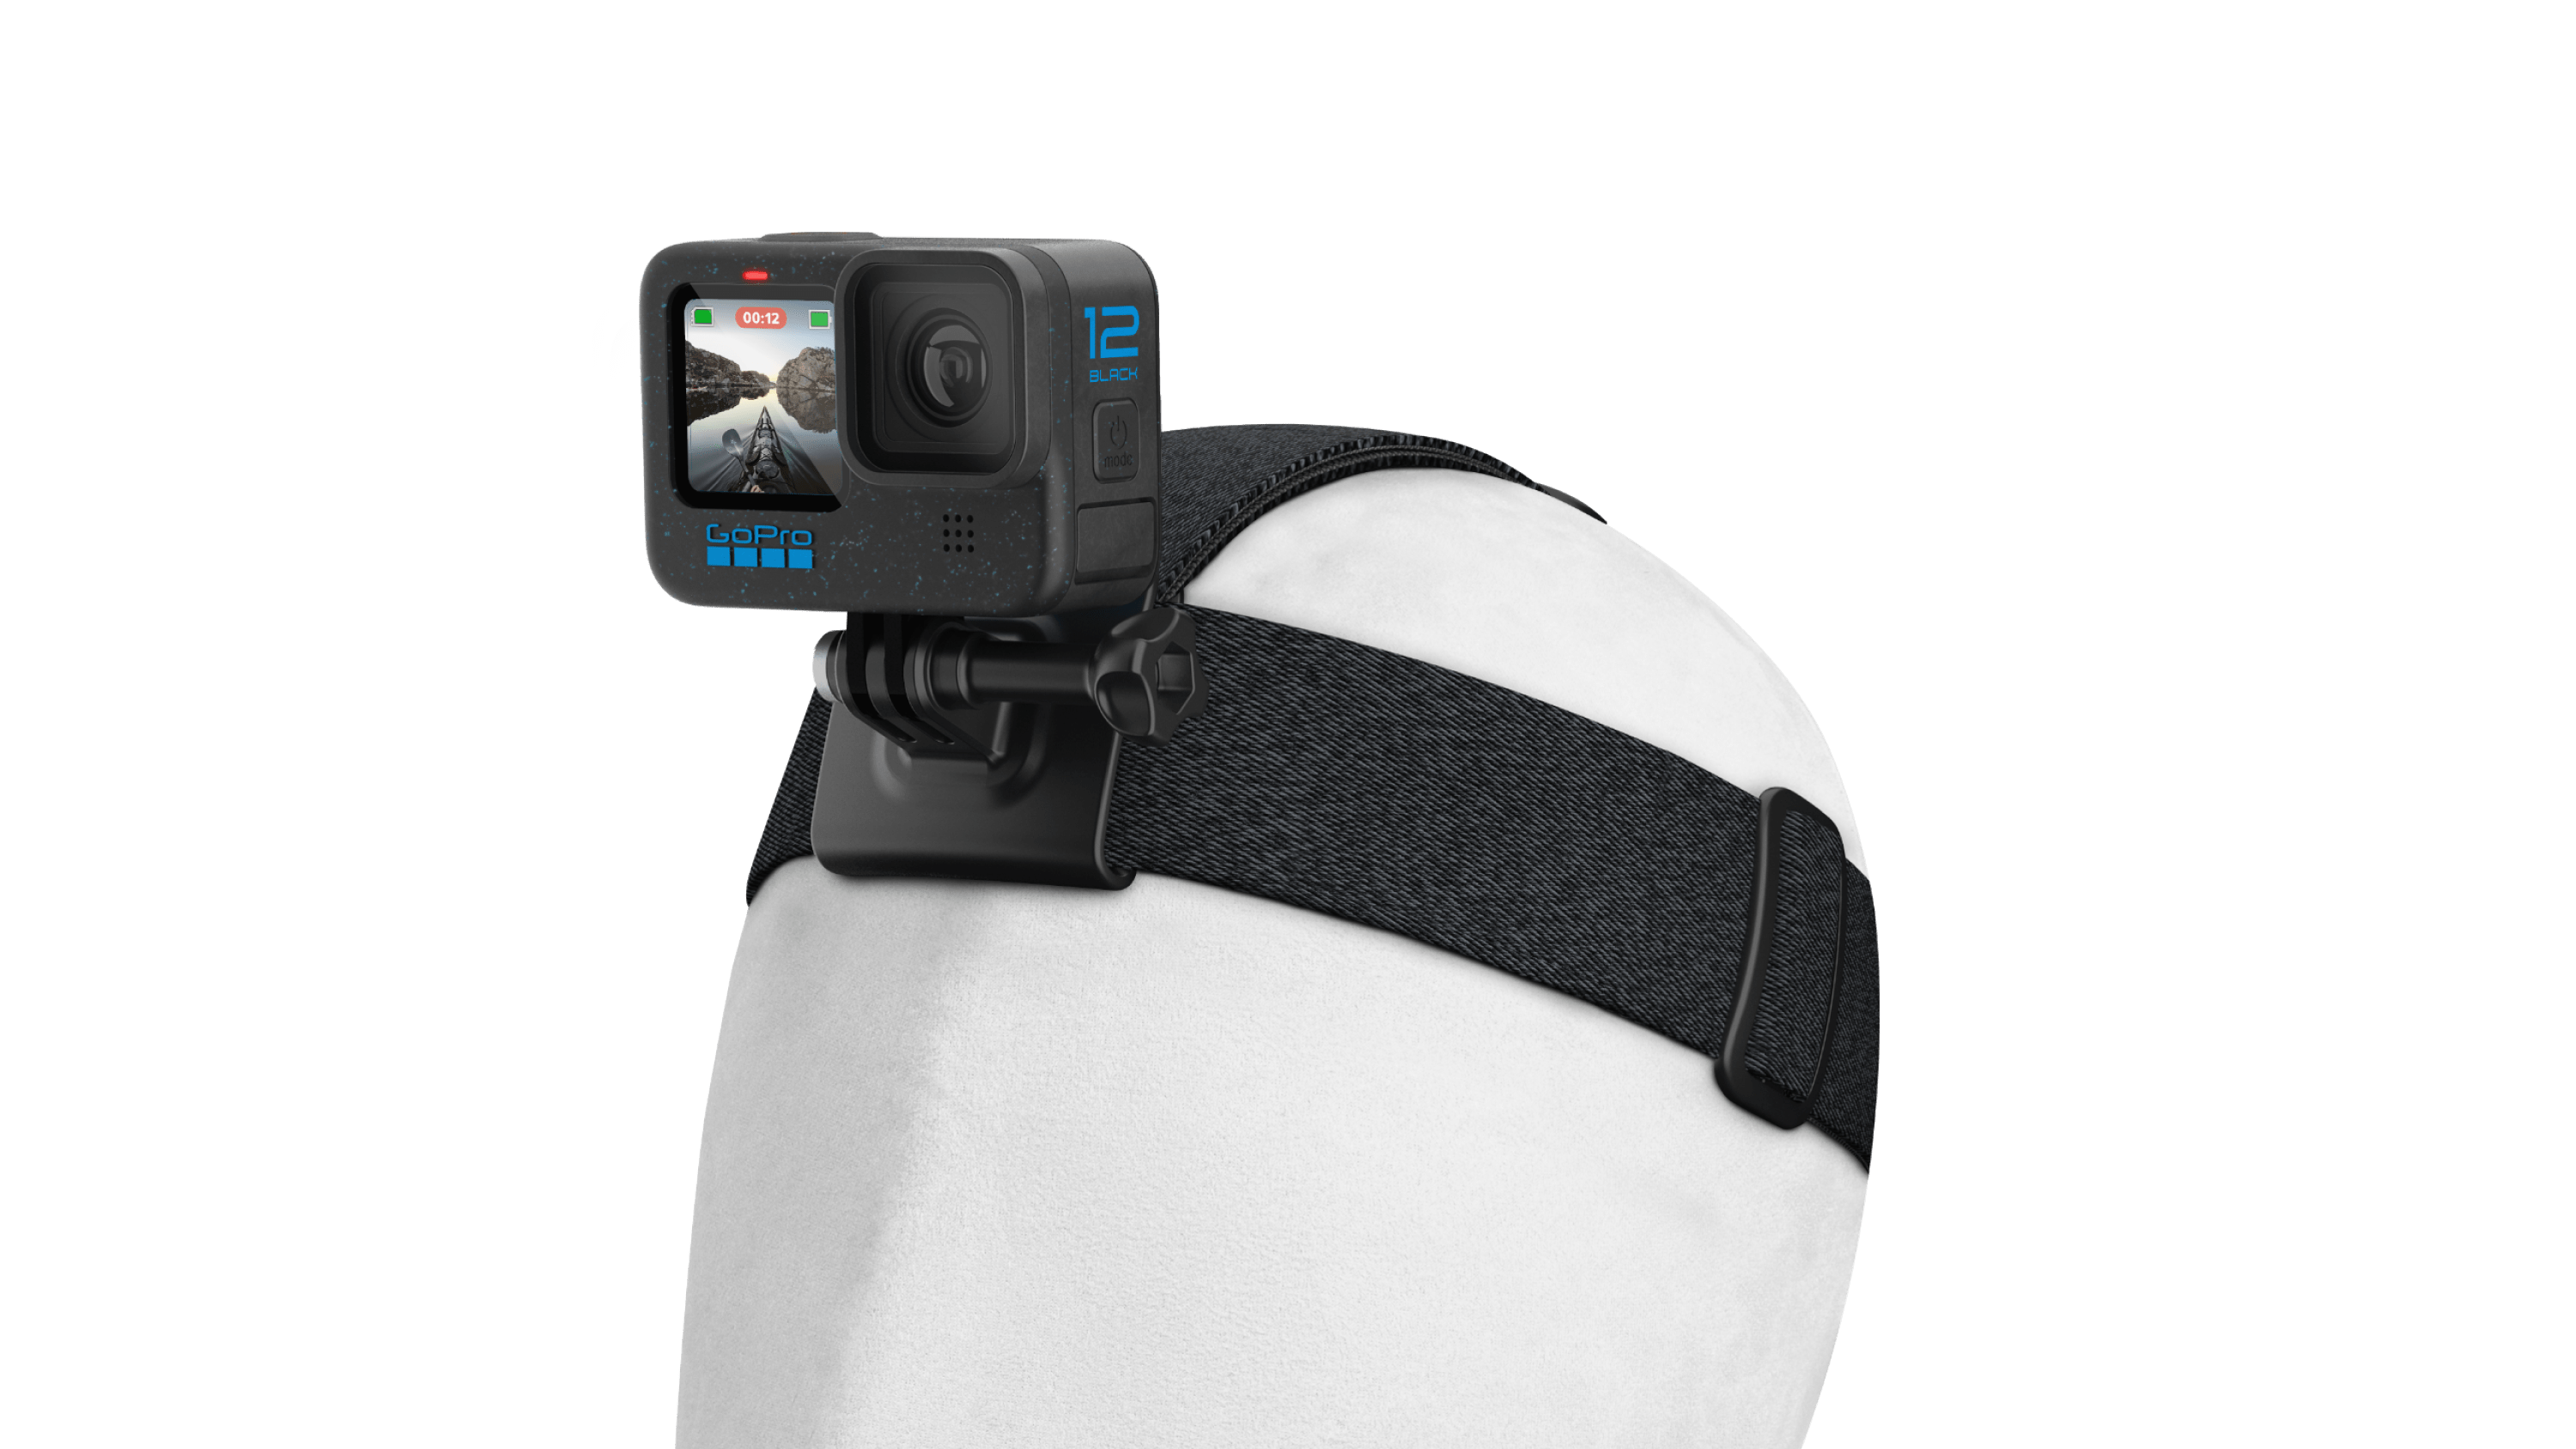
\includegraphics[width=\linewidth]{Images/gopro.png}\\
        (b) Action camera
    \end{minipage}
    \hfill
    \begin{minipage}{0.3\linewidth}
        \centering
        \includegraphics[width=\linewidth]{Images/bodycamera.png}\\
        (c) Body camera
    \end{minipage}
    \caption{Esempi di dispositivi indossabili per la cattura di video egocentrici}
    \label{fig:dispositivi_egocentrici}
\end{figure}

L'adozione di tali dispositivi è stata favorita dalla loro versatilità: da un lato vengono utilizzati per scopi ricreativi e per la condivisione di esperienze personali, dall'altro trovano applicazione in contesti professionali e industriali, dove consentono di documentare procedure complesse e migliorare i processi di formazione e supervisione. Ciò che rende peculiari i video egocentrici è la loro capacità di catturare dettagli e prospettive uniche, fornendo una visione diretta dell'attività di chi li indossa.

Il principale ostacolo all'analisi di questi contenuti risiede nella loro natura non strutturata. I video in prima persona possono essere considerati come veri e propri flussi di coscienza visivi: lunghi, frammentati, privi di un'organizzazione narrativa chiara e difficili da interpretare. La presenza di movimenti rapidi della fotocamera, variazioni di illuminazione e interazioni simultanee con più oggetti rende complicata l'estrazione di significato. Un'annotazione manuale completa non è praticabile, sia per la mole di dati prodotta sia per la complessità dei contenuti.

Da questa problematica emerge la necessità di costruire una “memoria artificiale” capace di trasformare i video egocentrici in rappresentazioni strutturate e interrogabili. Questa tesi prende avvio dall'analisi dei principali contributi degli elementi che vanno a formare un eventuale memoria artificiale, per poi focalizzarsi su AMEGO \cite{goletto2024amego}, acronimo di \emph{Active Memory of the EGOcentric video}, un sistema sviluppato per organizzare e rendere interrogabili i contenuti visivi in prima persona e attualmente considerato stato dell'arte nel suo ambito \cite{goletto2024amego}.

Il contributo di questo lavoro consiste nella valutazione di AMEGO in un contesto diverso rispetto a quello in cui è stato originariamente validato. Inizialmente il sistema è stato sperimentato sul dataset \emph{ EPIC KITCHENS }\cite{Damen2021PAMI}, una collezione di video ambientati in cucine domestiche. In questa tesi, invece, viene preso in esame il dataset \emph{ENIGMA-51} \cite{ragusa2023enigma51}, un dataset egocentrico acquisito in scenari industriali, in cui diversi operatori hanno seguito procedure guidate per eseguire attività di riparazione di quadri elettrici. La differenza tra i due domini rende lo studio particolarmente interessante, in quanto consente di valutare la capacità di AMEGO di generalizzare a contesti applicativi mai visti.

In ambito industriale, l'analisi dei video egocentrici e la gestione della concurrency assumono un ruolo fondamentale per ottimizzare diversi aspetti operativi. In particolare, si possono individuare due benefici principali:
\begin{itemize}
    \item \textbf{Affidabilità del processo:} garantire che le operazioni vengano eseguite nell'ordine corretto consente di ottimizzare i flussi produttivi e di ridurre il rischio di errori umani, assicurando maggiore coerenza nelle procedure.
    \item \textbf{Sicurezza dei lavoratori:} monitorare in tempo reale l'uso corretto dei dispositivi di protezione individuale (DPI) oppure verificare la collocazione di componenti critici. Ad esempio, un materiale pericoloso come un condensatore ad alta tensione deve essere riposto in aree designate per prevenire incidenti.
\end{itemize}

Un aspetto centrale analizzato in questo lavoro riguarda la gestione della \emph{concurrency}, intesa come la capacità di riconoscere non solo con quali altri oggetti un determinato strumento viene utilizzato in simultanea, ma anche in quali contesti o aree operative tale oggetto viene impiegato.
Nei capitoli successivi verranno prima esaminati gli strumenti e le metodologie attualmente presenti in letteratura, che costituiscono le basi per lo sviluppo di sistemi di memoria artificiale per video egocentrici. Successivamente saranno illustrate nel dettaglio le caratteristiche di AMEGO \cite{goletto2024amego} e le sperimentazioni condotte sul dataset ENIGMA-51 \cite{ragusa2023enigma51}, con l'obiettivo di valutare fino a che punto il sistema possa essere adattato a contesti applicativi diversi da quelli per cui è stato originariamente progettato.